In this Section we detail the process of gathering data from the
subjects and processing them in order to make them suitable for
analysis by a Support Vector Machine. The aim is that of building
sequences of biometric data (hand position and posture) from time
sequences in which the times of start and end of the grasps are
unknown.

\subsection{Experimental Setup}

\subsubsection*{Devices}

We collected data using a 22-sensors Immersion DataGlove for the hand
posture \cite{dataglove}, an Ascension Flock-Of-Birds (FoB) for the hand
position \cite{fob} and a Force Resistor Sensor (FSR) to detect the
contact moment with the object. Figure \ref{fig:devices} shows the
devices, as worn by a subject.

\begin{figure}[htbp]
  \begin{center}
    \begin{tabular}{cc}
      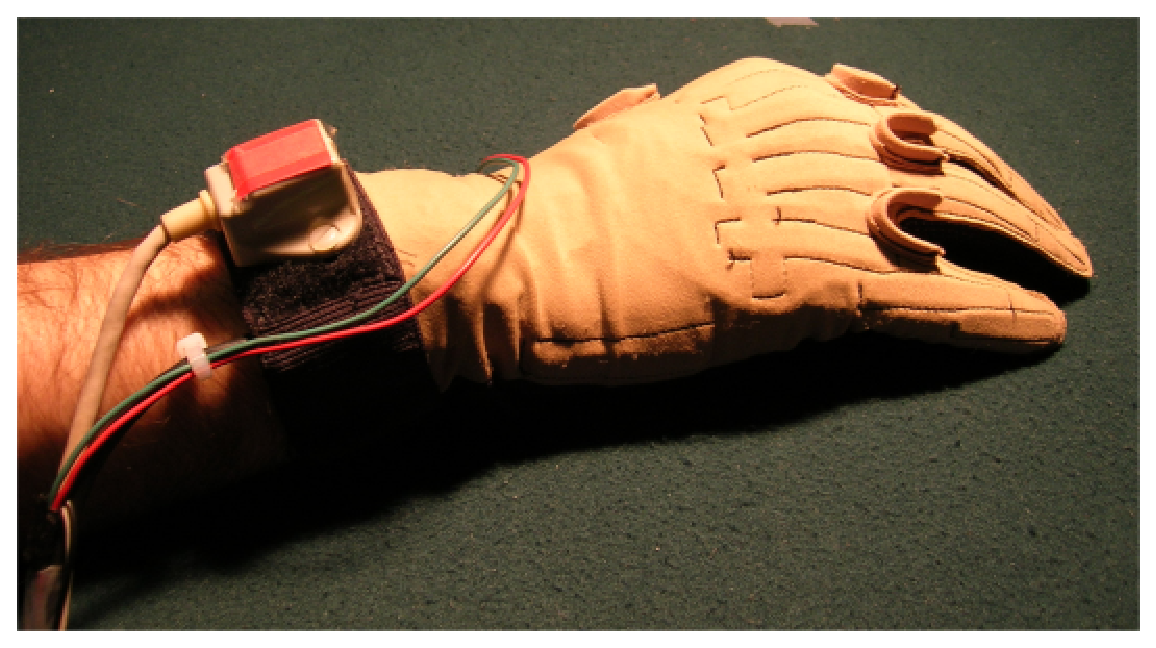
\includegraphics[width=0.45\linewidth]{devices1.eps} &
      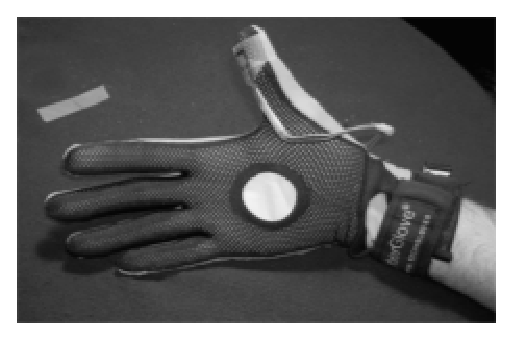
\includegraphics[width=0.45\linewidth]{devices2.eps} \\
      $(a)$ & $(b)$
    \end{tabular}
    \caption{The devices used for the experiment, as worn by a
    subject: $(a)$ the DataGlove with the Flock-of-Birds just above the
    subject's wrist; $(b)$ the Force Resistor Sensor attached to the
    subject's thumb.}
    \label{fig:devices}
  \end{center}
\end{figure}

The DataGlove was worn by the subject on the right hand. The device
returns $22$ $8$-bit numbers linearly related to the angles between
the ends of the sensors and roughly indicating the angles between the
subject's hand joints; the sensors are embedded in the glove in order
for them to be adherent to the subject's skin. The resolution of the
sensors is on average about $1$ degree \cite{dataglove_res}. The
sensors describe the position of the three phalanxes of each finger
(for the thumb, rotation and two phalanxes), the four finger-to-finger
abductions, the palm arch, the wrist pitch and the wrist yaw.

The FoB was firmly mounted on the DataGlove, just above the subject's
wrist, with the X/Y plane being parallel to the palm plane in the
resting position. The device returns $6$ double-precision numbers
describing the position ($x$, $y$ and $z$ in inches) and rotation
(azimuth, elevation and roll in angles) of the sensor with respect to
a magnetic basis mounted about one meter away from the subject. The
FoB's resolution is about $??$ \cite{fob_res}.

Lastly, the FSR was mounted on the subject's thumb. It returns a
$32$-bit number approximately inversely proportional to the pressure
applied to the surface of the sensor.

All data were synchronised, collected and saved in real time at about
$50$Hz.

\subsubsection*{Subjects}

Eleven subjects, four females and seven males aged $24$ to $34$ of
several different nationalities, joined the experiment. They were all
right-handed and fully able-bodied, and were given initially some
knowledge of the aim of the experiment.

\subsubsection*{Method}

The subjects were asked to sit confortably in front of a clean
workspace of about one squared meter, at the center of which an object
was placed, in a predefined position. The subjects were then asked to
wear the devices and choose a resting position for their right hand
and arm. They were then instructed to grasp the object with their
right hand any way they wanted, not necessarily the same way each
time, keeping a ``natural'' attitude. After grasping the object, they
had to drop it somewhere else in the workspace, and then return their
right hand and arm in the initial resting position. Subsequently, they
had to use their left hand to reposition the object roughly in the
same place it was before.

We first had the subjects do a trial run of the experiment, in order
for them to gain confidence in the setup. A beeping sound was heard
each time the subject made contact with the object (that is, each time
the FSR signalled a significant change), and they were asked to try
and hear the beep each time they grasped the object. Although this
ruled out grasps which made no use of the thumb, it enabled us to
better gather the contact points.

After the trial run, subjects were asked to repeat the
grasp/drop/reposition procedure $120$ times per each object. We
employed, in turn, three objects: a beer can, a scotch tape roll and a
mug (Figure \ref{fig:objects} shows the objects).

\begin{figure}[htbp]
  \begin{center}
    \begin{tabular}{ccc}
      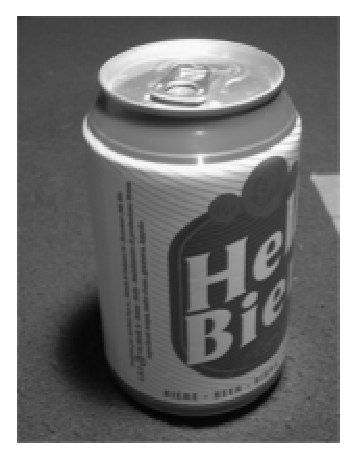
\includegraphics[height=0.2\textheight]{beer.eps} &
      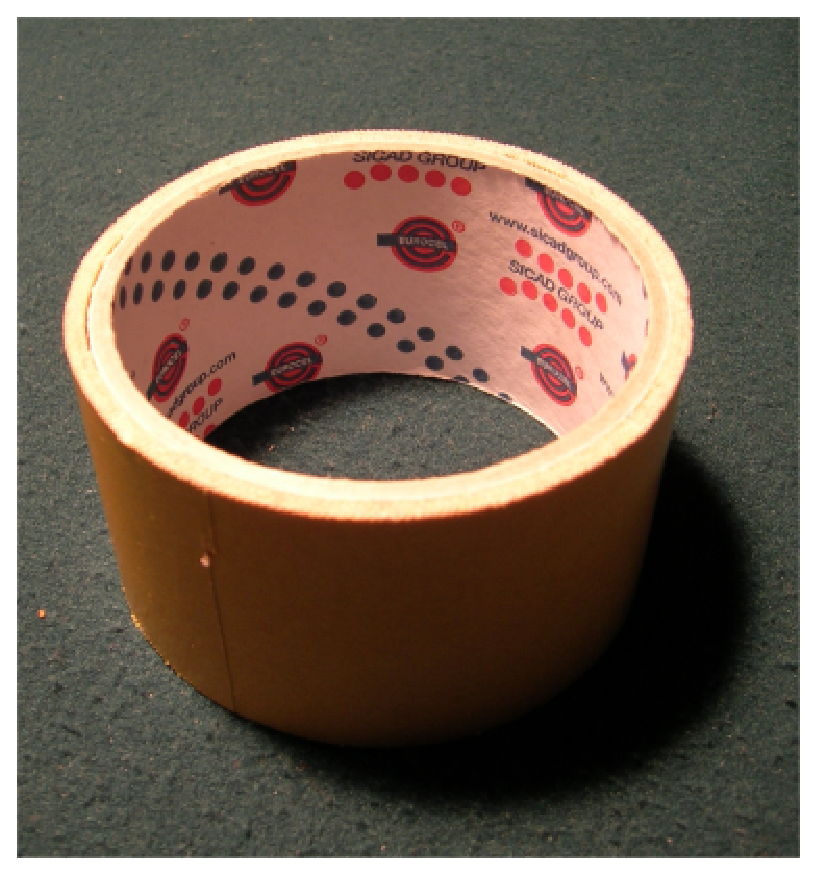
\includegraphics[height=0.2\textheight]{scotch.eps}  &
      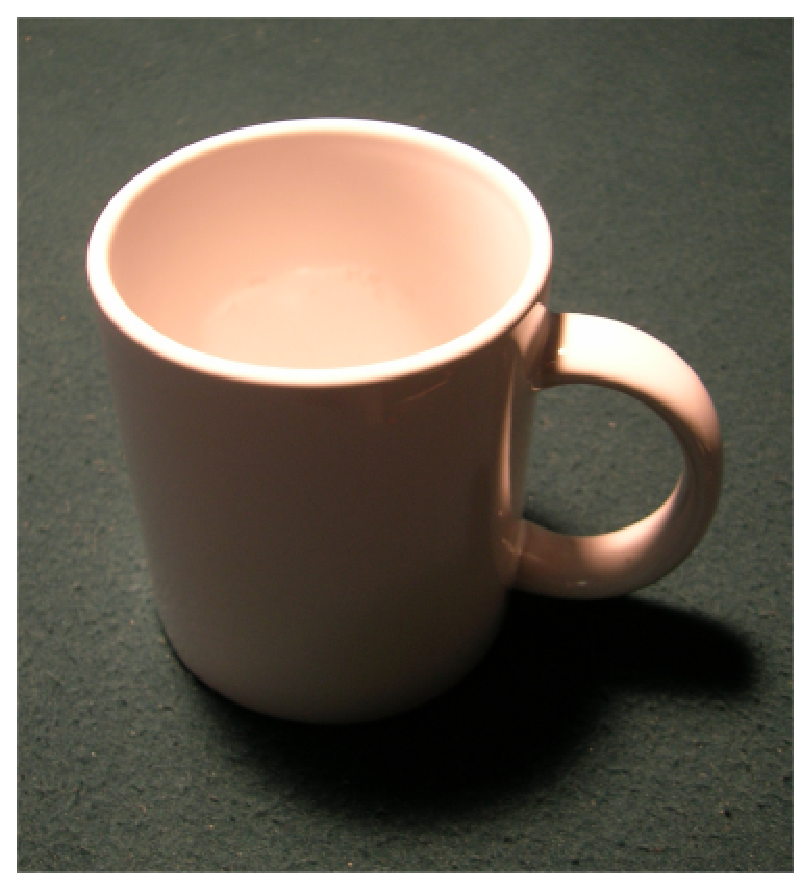
\includegraphics[height=0.2\textheight]{mug.eps} \\
      $(a)$ & $(b)$ & $(c)$
    \end{tabular}
    \caption{The objects used inthe experiment: a beer can $(a)$, a scotch
    tape roll $(b)$ and a mug $(c)$.}
    \label{fig:objects}
  \end{center}
\end{figure}

The $120$-grasps session was done twice, resulting in approximately
$240$ grasps for each of the three objects. The numbers are not
precise since now and then the subjects would grasp without properly
activating the FSR. This problem has been corrected in the batch
analysis of data. Moreover, in two cases the FSR broke down toward the
end of the experiment, resulting in a slightly smaller number of
grasps. In order not to have the subjects ``specialise'' on a
particular object, we alternated the sessions this way: first the can,
then the roll and then the mug, all of this two times.

Each experiment (one subject, six sessions) lasted $35$ to $56$
minutes depending on the subject's confidence and speed; although
almost no subjects reported tiredness, we allowed for rest between
each session. It was reported by almost every subject that the
experiment became rapidly boring, which lets us claim that almost all
grasps were done in a natural, almost unconscious way. Figure
\ref{fig:setup} shows the main phases of the experiment.

\begin{figure}[htbp]
  \begin{center}
    \begin{tabular}{ccc}
      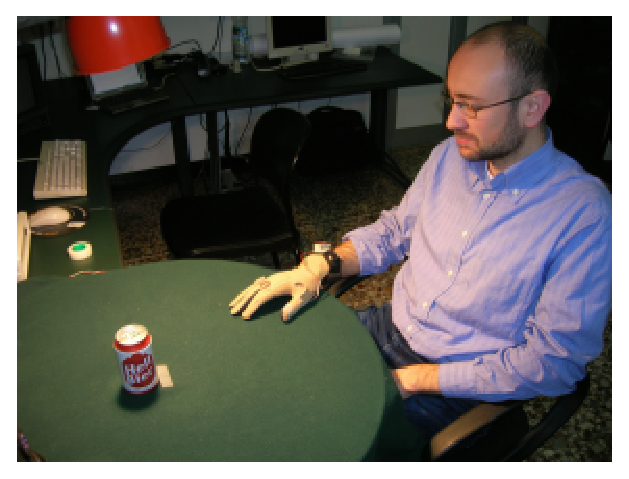
\includegraphics[width=0.3\linewidth]{exp1.eps} &
      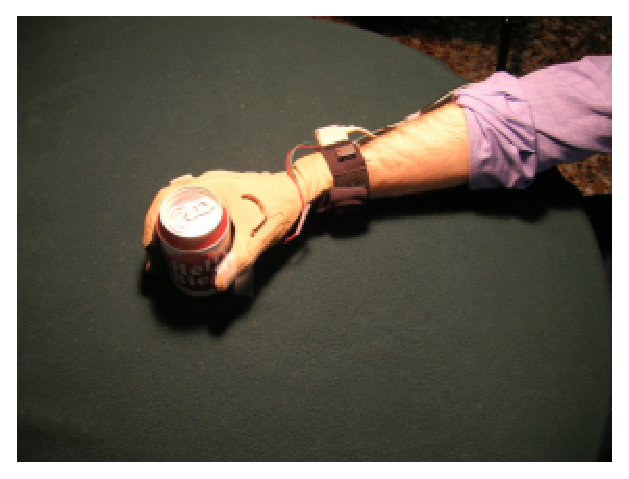
\includegraphics[width=0.3\linewidth]{exp2.eps}  &
      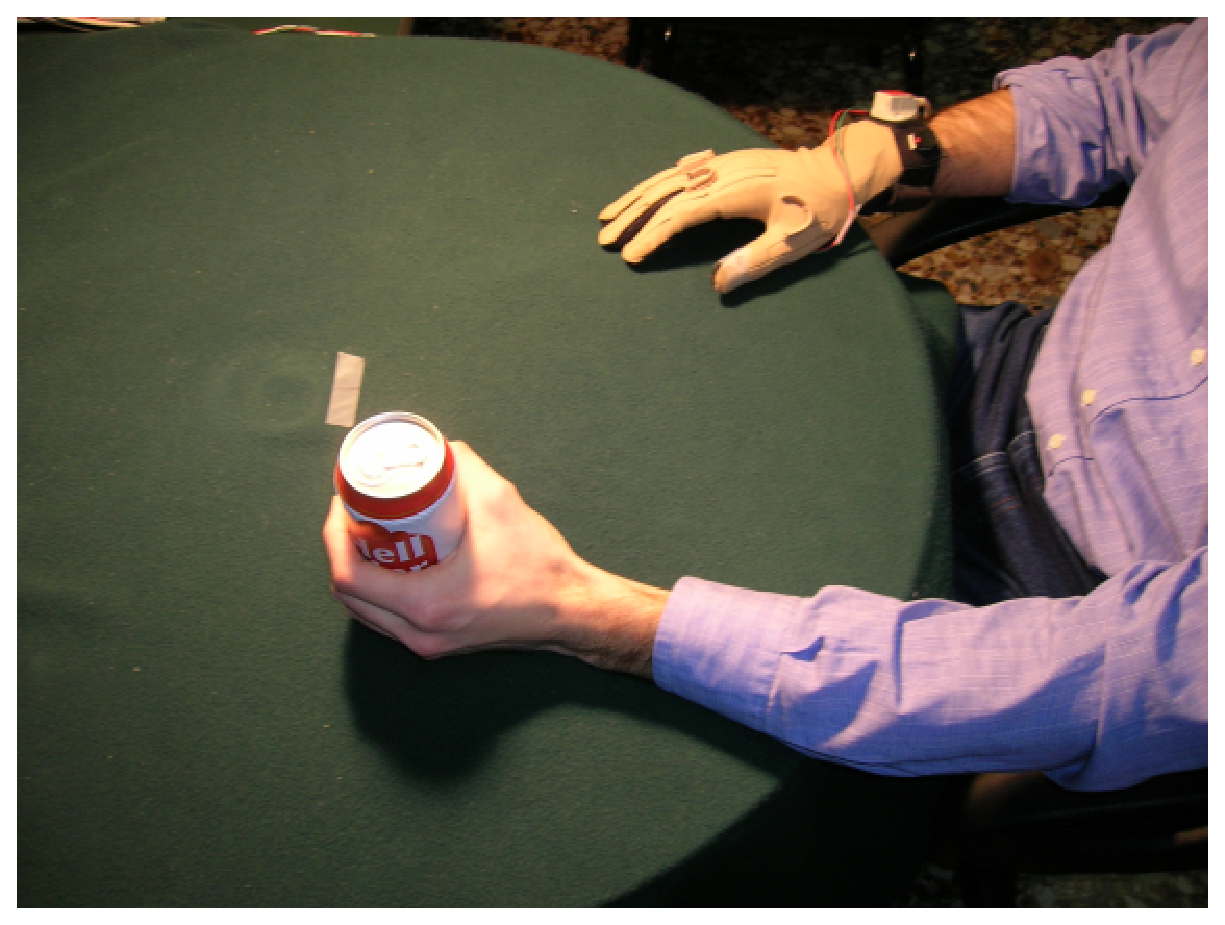
\includegraphics[width=0.3\linewidth]{exp3.eps} \\
      $(a)$ & $(b)$ & $(c)$
    \end{tabular}
    \caption{The experiment. The subject sits confortably in front of
    a clean workspace, at the center of which an object is placed
    $(a)$, with his right hand in a resting position. He then grasps
    the object and drops it somewhere else in the workspace $(b)$,
    bringing then his arm and hand in the resting position. Lastly, he
    repositions the object in the initial position using his left arm
    and hand $(c)$. The procedure is repeated for $120$ times, then
    this session is repeated for each of the three objects, and all of
    this is done twice, resulting in approximately $240$ grasps for
    each subject and object.}
    \label{fig:setup}
  \end{center}
\end{figure}

\subsection{Building the training set}

\subsubsection*{Detecting grasps}

In order to train a Support Vector Machine, it is required that an
appropriate number of \emph{examples} be extracted from the subjects'
data. An example in this setting is a time sequence of biometric data,
gathered off a single joint, together with a target value for that
joint --- the value the SVM must guess by means of regression.

As described above, each user was instructed to grasp each object in
two separate sessions; therefore, each session records a time sequence
in which data from all sensors ($6$ from the FoB and $22$ from the
DataGlove) are recorded continually. From each session and for each
sensor we have automatically extracted the sub-sequences representing
the grasping action.

In order to figure out when each single grasping sequence starts and
ends, we first observed the values of the FSR mounted on the subject's
thumb. We manually verified that the FSR correctly reacted in almost
all cases with a spike, signalling, whenever the subject made contact
with the object, a significantly different value from that recorded
elsewhere shortly before the contact. The spike instants were taken as
the \emph{ending} points of each grasp sequence, and were gathered by
checking when the first derivative of its value dropped by more than
$10\%$ of its overall minimum value. Moreover, after each spike, we
ignored one second of the sequence, in order not to detect possible
spurious spikes which happened immediately after the grasp, due to
object slippage and/or blurred values coming from the FSR.

Subsequently, in order to detect the \emph{starting} point of each
grasp, for each ending point, we observed the hand speed and
acceleration, averaged over $0.2$ seconds, from the ending point
backwards. Since we had instructed the subjects to always return to
the resting position before initiating a new grasp, when the grasp
starts, the speed must be close to zero and the acceleration must be
negative (the subject's arm is moving \emph{toward} the FoB's
reference point). Therefore, we set the grasp starting point at the
nearest moment in time before the ending point in which the hand speed
was close to zero and the hand acceleration was negative. In order to
avoid detecting spurious speed/acceleration glitches when the hand
made contact with the object, we ignored $0.1$ seconds just before the
ending point. Figure \ref{fig:grasp_detection} $(a)$ shows an example
set of detected grasps. The detected start and end points of the
grasps are highlighted. As one can see, the hand speed (green curve)
shows the well known bell-shaped curve during a grasp \cite{...} {\bf
GIORGIO metti una citazione qui}: the hand speed diminishes, reaches a
minimum and then gets back to zero till the ending point of the grasp.

\begin{figure}[htbp]
  \begin{center}
    \begin{tabular}{ccc}
      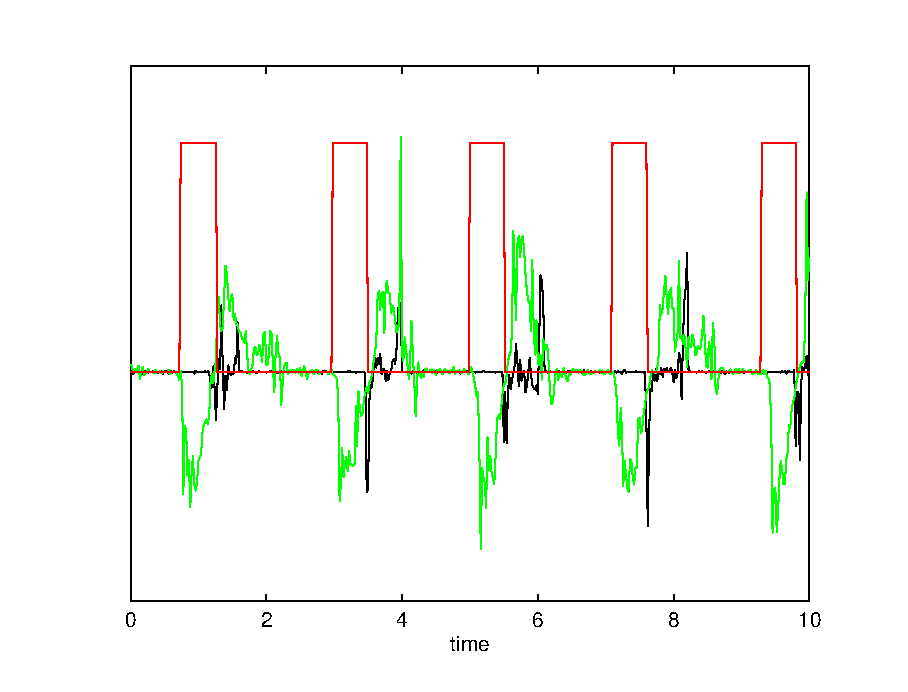
\includegraphics[width=0.48\linewidth]{grasp_seq_scotch.eps} &
      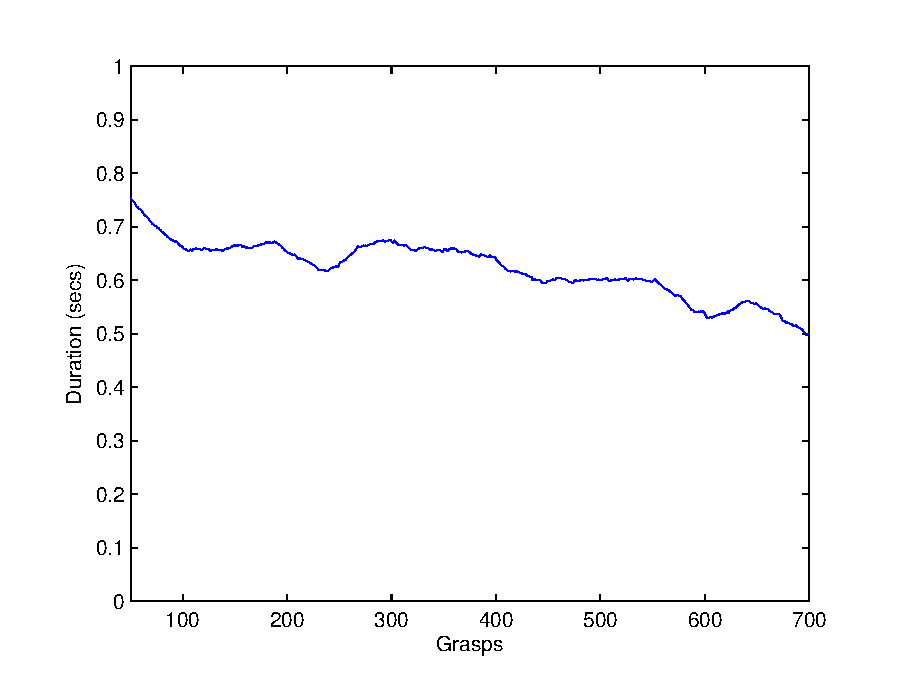
\includegraphics[width=0.48\linewidth]{grasp_trend.eps} \\
      $(a)$ & $(b)$
    \end{tabular}
    \caption{$(a)$ Detecting the grasps. The Figure shows $10$ seconds
    of the subject grasping an object. The red bands indicate the
    start and end of a grasp; the black line is the FSR response; and
    the green line is the hand speed. As one can see, the ending
    points are found near the FSR spike, indicating contact; moreover,
    the hand speed shows the well known bell-shaped curve during a
    grasp. $(b)$ Grasps duration. The Figure shows the speed of the grasps
    (moving average over 50 grasps) averaged for all subjects. As the
    experiments advance, the grasping durations become shorter and
    shorter.}
    \label{fig:grasp_sequence}
  \end{center}
\end{figure}

Overall, the procedure could recognise $727 \pm 9$ grasps for each
subject, which matches the desired result of $720$, that is, $120$ per
session with two sessions and three objects. As far as the two
subjects who broke down the FSR, the procedure recognised $565$ and
$658$ grasps. The data were also manually observed in order to verify
that spurious detected grasps would be an insignificant fraction of
the total grasps.

\subsubsection*{Grasping speed}

In order to make time sequences suitable for Support Vector Machines,
they must be all the same length\footnote{an interesting possbility is
that of employing a kernel which can consider time sequences of
different lenghts, see e.g. \cite{...} {\bf FRANCESCO aggiungi
citazione qui}. This issue is the subject of future research.}; in
order to do this, since in general not all grasp sequences have the
same length, it is crucial to have an idea of how fast the grasps are.
Figure \ref{fig:grasp_sequence} $(b)$ shows the average grasp
durations for all subjects over the six sessions of each experiment
(moving average over $50$ grasps); as one would expect, in general the
subjects get rapidly used to the grasp/drop/reposition task and the
grasps become faster and faster. It must be remarked, though, that
this is not the case for all subjects considered one by one. Overall,
the grasps last $0.61 \pm 0.21$ seconds.

Therefore, we stretched every grasp sequence to $1$ second by linear
interpolation, obtaining fixed-length time sequences of $50$ samples
for each sensor and grasp sequence.
